\chapter{Разработка модуля расчета мощности дозы внешнего гамма - излучения}
\label{chapter_dose}

\section{Необходимость расчета мощности дозы гамма - излучения}
\label{sec_gamma_theory}

Радиоактивные нуклиды, которые могут попасть в атмосферу в результате аварии на \ac{aes}, являются бета-активными. При 
протекании бета-распада результирующее ядро может оказаться в возбужденном состоянии. Возбуждение ядра снимается 
посредством испускания гамма - квантов. Для примера, на рисунке \ref{fig_I_133_decay_gamma} представлена упрощенная схема 
распада изотопа $^{131}I$, после которого образуется изотоп $^{131}Xe$ в возбужденном состоянии, испускающий 
гамма - кванты при переходе в основное состояние.

\begin{figure}[ht!]
    \centering
    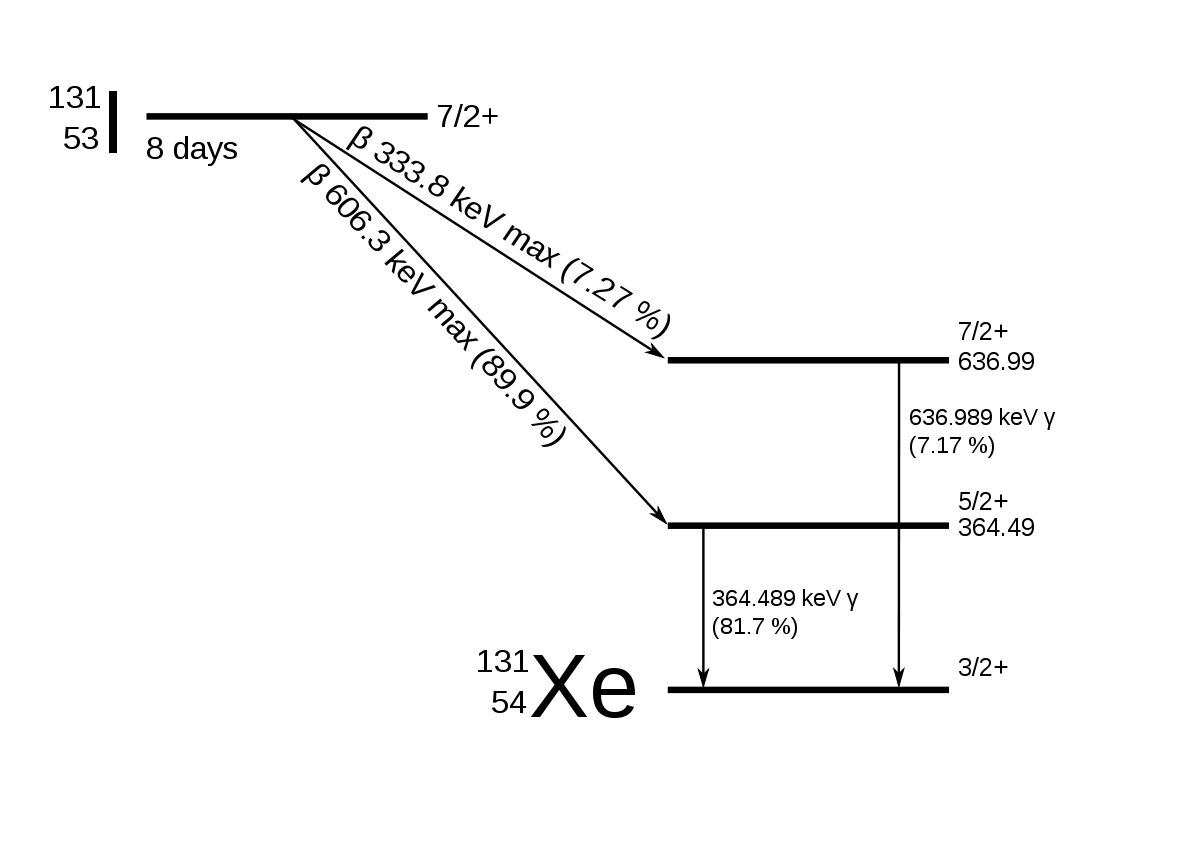
\includegraphics[width=13cm]{I_133_decay_gamma}
    \captionsetup{justification=centering}
    \caption{Упрощенная схема распада изотопа $^{131}I$.}
    \label{fig_I_133_decay_gamma}
\end{figure}

Одной из главных задач современных систем \ac{ascro} на \ac{aes} является измерение значений мощности дозы 
гамма - излучения на прилегающей к \ac{aes} местности. Значение мощности дозы гамма - излучения на местности необходимо знать 
для контроля радиационной обстановки вокруг \ac{aes}, а также своевременной выдаче рекомендаций по принятию решений о 
защите населения. Измерение мощности дозы гамма - излучения в системах \ac{ascro} проводится при помощи 
специализированных датчиков радиационного контроля, расположенных на прилегающей к \ac{aes} местности. 

\section{Датчики радиационного контроля}

Основу \ac{ascro} составляет система постов радиационного контроля гамма - излучения, расположенных вокруг \ac{aes}. 
Обычно, измерительные блоки фотонного излучения содержат датчики двух диапазонов: $10^{-7}$ - $10^{-3}$ Зв и $10^{-3}$ 
- $10$ Зв. В качестве блоков детектирования в системах постов радиационного контроля \ac{ascro} используются БДМГ-08Р3, 
БДМГ-08Р4, БДМГ-08Р5, БДМГ-100 \cite{elokhin}. Для примера, рассмотрим технические характеристики блока детектирования 
БДМГ-100.

Блок детектирования БДМГ-100 предназначен для непрерывного измерения \ac{maed} (\acl{maed}) \cite{bdmg-100}. Блок 
применяется для контроля радиационной обстановки на объектах атомной энергетики и радиохимического производства; на 
промышленных предприятиях, использующих источники ионизирующих излучений; на пунктах специального и таможенного контроля 
и в службах экологического и санитарно-эпидемиологического надзора. В таблице \ref{table_bdmg_100} приведены основные 
техническите характеристики блока детектирования БДМГ-100.

\begin{table}[ht]
	\setlength{\extrarowheight}{1mm} 
	\caption{Основные технические характеристики блока детектирования БДМГ-100 \cite{bdmg-100}.}
	\label{table_bdmg_100}
	\centering
    \begin{tabular}{|M{0.6\textwidth}|M{0.3\textwidth}|}
    \hline Характеристика & Значение \\
    \hline Диапазон энергий регистрируемого гамма - излучения & от 0,05 до 3,0 МэВ \\
    \hline Диапазон измерений МАЭД гамма - излучения в чувствительном поддиапазоне & от 0,1 мкЗв/ч до 2 мЗв/ч \\
    \hline Диапазон измерений МАЭД гамма - излучения в грубом поддиапазоне & от 0,5 мЗв/ч до 10 Зв/ч \\
    \hline Пределы допускаемой основной относительной погрешности измерений МАЭД гамма - излучения & $\pm$(15 + 3/Н*) \% \\
    \hline Время установления рабочего режима блока & не превышает 1 мин \\
    \hline Время непрерывной работы & не ограничено \\
    \hline Напряжение питания постоянного тока & 12 $\pm$ 0,5 В \\
    \hline \makecell{Потребляемый ток при напряжении \\ питания 12 В} & не более 25 мА \\
    \hline Температура окружающего воздуха & от -40 до +50 °С \\
    \hline Относительная влажность окружающего воздуха & до 98 \% при +35 °С \\
    \hline Атмосферное давление & от 84,0 до 106,7 кПа \\
    \hline 
    \end{tabular}
\end{table}

Принцип работы блока БДМГ-100 основан на преобразовании энергии ионизирующих излучений в электрические импульсы. В 
качестве детекторов ионизирующего излучения в блоках БДМГ-100 используются газоразрядные счетчики Гейгера-Мюллера, а 
именно: для чувствительного поддиапазона 2 счетчика СБМ20, а для грубого поддиапазона один счетчик Гамма-1 (СИ-34Г). На 
рисунке \ref{fig_bdmg_100} представлены габаритные и присоединительные размеры блока БДМГ-100.

\begin{figure}[ht!]
    \centering
    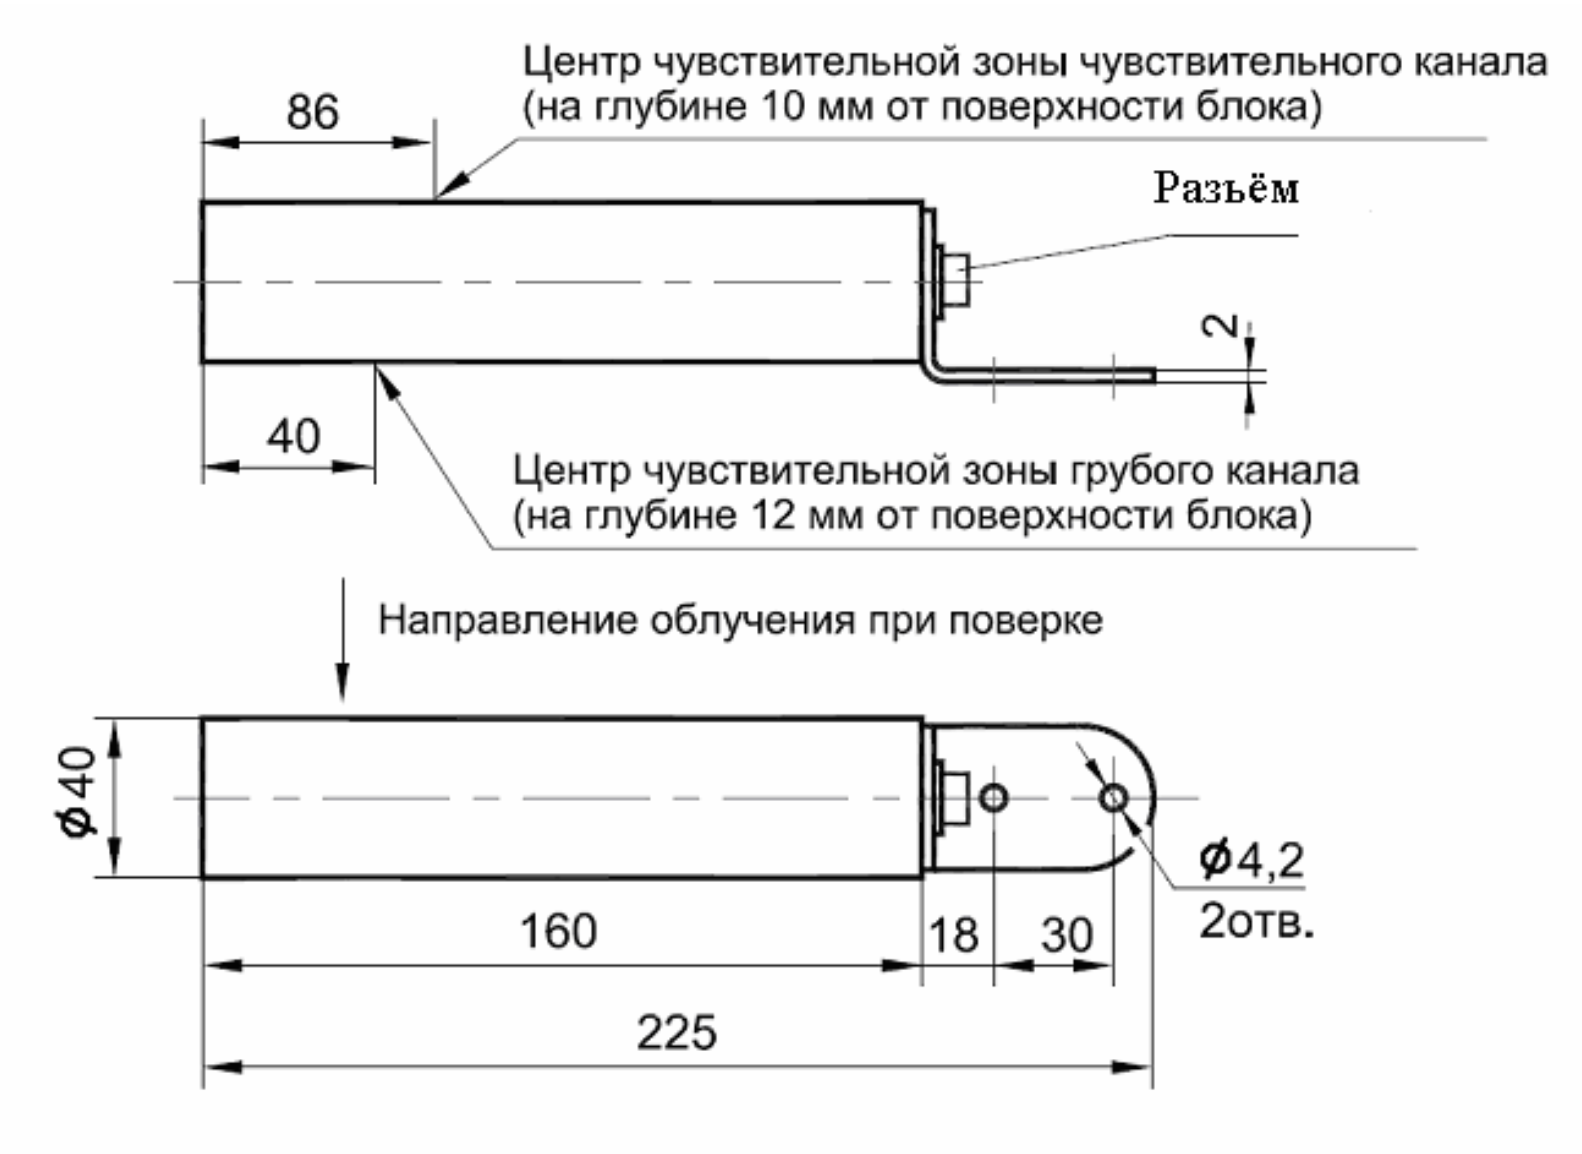
\includegraphics[width=13cm]{bdmg-100}
    \captionsetup{justification=centering}
    \caption{Габаритные и присоединительные размеры блока БДМГ-100 \cite{bdmg-100}.}
    \label{fig_bdmg_100}
\end{figure}

Измерение мощности дозы гамма - излучения в системах \ac{ascro} выполняется при помощи датчиков радиационного контроля, 
размещенных вокруг \ac{aes}. Одной из важнейших задач проектирования систем \ac{ascro} является их оптимизация. Под 
оптимизацией \ac{ascro} понимается выбор необходимого и достаточного количества датчиков радиационного контроля, 
размещенных вокруг \ac{aes}, а также методы их размещения, при помощи которых можно повысить точность прогностических 
расчетов при оценке уровней радиационного загрязнения подстилающей поверхности, дозовых нагрузок на персонал и население 
в случае радиационной аварии.

\section{Оптимизация количества датчиков радиационного контроля}

При проектировании систем \ac{ascro} ставится задача обеспечения наибольшей точности измерений и контроля радиационного 
загрязнения внешней среды. 

Основным средством измерения \ac{ascro} являются гамма - датчики. К размещению гамма - датчиков на прилегающей к \ac{aes} 
местности ставятся демографические, экономические и экологические требования. Демографические требования учитывают 
численность населения - пост контроля устанавливается в населенном пункте с численностью населения более 5 тыс. человек. 
Гамма - датчики требуют для нормальной работы основные и дополнительные линии связи электрического питания, автономного 
питания и другого оборудования, стоимость которых определяет главные затраты на систему. В связи с этим возникает 
экономическое требование - уменьшение количества постов (датчиков) радиационного контроля. С точки зрения экологии 
важно знать точную информацию об уровне загрязнения окружающей среды вблизи \ac{aes} при любом направлении выброса, что 
достигается увеличением числа постов радиационного контроля.

Таким образом, ставится задача оптимизации числа датчиков радиационного контроля с демографической, экономической и 
экологической точек зрения.

В таблице \ref{table_aes_ascro} приведено количество постов радиационного контроля на российских \ac{aes}. Из таблицы 
видно, что количество постов радиационного контроля на российских \ac{aes} различается. Кроме того, в каждом из случаев 
количество постов научно необоснованно с точки зрения оптимальности, описанной выше. Это связано с недостаточным 
финансированием по федеральной программе «Ядерная и радиационная безопасность России» на создание \ac{ascro} 
на действующих \ac{aes} \cite{elokhin}.

\begin{table}[ht]
	\setlength{\extrarowheight}{1mm} 
	\caption{Количество постов радиационного контроля на российских \ac{aes} \cite{elokhin}.}
	\label{table_aes_ascro}
	\centering
    \begin{tabular}{|M{0.3\textwidth}|M{0.3\textwidth}|}
    \hline \ac{aes} & Кол-во постов контроля \\
    \hline Балаковская & 25 \\
    \hline Белоярская & 8 \\
    \hline Билибинская & 10 \\
    \hline Калининская & 18 \\
    \hline Кольская & 20 \\
    \hline Курская & 29 \\
    \hline Ленинградская & 14 \\
    \hline Нововоронежская & 22 \\
    \hline Ростовская & 19 \\
    \hline Смоленская & 18 \\
    \hline 
    \end{tabular}
\end{table}

Рассмотрим принцип определения необходимого и достаточного количества датчиков, описанного в работе \cite{kummel_opt}.
В качестве дозовых критериев выбирается мощность дозы внешнего облучения, а в качестве порога - мощность дозы внешнего 
облучения для населения.

Положим, что радиоактивный выброс распространяется с высоты $h_{ef}$ при наихудших метеорологических условиях. Согласно
модели Пасквилла – Гиффорда \cite{atmos_doc} такие условия соответствуют классу устойчивости атмосферы типа F (сильный
ветровой перенос и слабая поперечная диффузия выброса). Задается расстояние $R$, которое обычно выбирается исходя из 
радиуса \ac{szz} (\acl{szz}) \ac{aes}. Задается мощность дозы внешнего облучения на расстоянии $R$ от источника выброса, 
равная предельно-допустимой мощности дозы для населения, предполагая, что такую мощность создает радиоактивный выброс на 
расстоянии $R$ от источника.

На подстилающей поверхности рассчитывается распределение мощности дозы внешнего облучения в направлении, 
перпендикулярном к радиусу (рисунок \ref{fig_det_opt}), считая, что на границе \ac{szz} достигается предельно допустимая
мощность дозы. По полученному распределению находят расстояние $\delta$, на котором мощность дозы равна порогу 
чувствительности датчика. Используя полученное расстояние, необходимое число датчиков определяют целой частью отношения 
\ref{eq_n_detectors}.

\begin{equation}
    \label{eq_n_detectors}
    N_n = [\frac{2 \pi R}{2 \delta}] = [\frac{\pi R}{\delta}]
\end{equation}

Достаточное число датчиков определяется по формуле \ref{eq_d_detectors}.

\begin{equation}
    \label{eq_d_detectors}
    N_a = N_n + 1
\end{equation}

Считая $R = 3$ км, а класс устойчивости атмосферы типа F, необходимое количество датчиков составляет 22-24. При другом классе
устойчивости атмосферы, к примеру A, когда ветровой перенос радиоактивной примеси невелик, но значительна поперечная диффузия
примесей, необходимое количество датчиков составляет 14-16.

\begin{figure}[ht!]
    \centering
    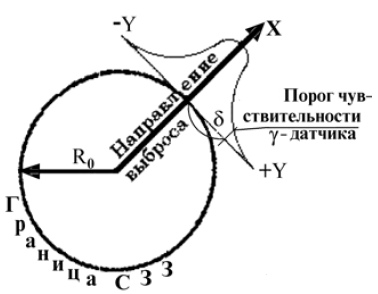
\includegraphics[width=9cm]{det_opt}
    \captionsetup{justification=centering}
    \caption{Выбор оптимального количества датчиков \ac{ascro} \cite{elokhin}.}
    \label{fig_det_opt}
\end{figure}


В итоге можно сделать вывод о том, что наименьшее число датчиков должно рассчитываться исходя из наихудших метеорологических
условий (класс устойчивости атмосферы типа F) по формуле \ref{eq_d_detectors}. Важно отметить, что с уменьшением порога 
чувствительности детекторов гамма - излучения увеличивается параметр $\delta$, что влечет за собой уменьшение наименьшего
количества датчиков без потери чувствительности системы в целом.

\section{Методика расчета мощности дозы гамма - излучения}

Рассмотрим методику расчета мощности эквивалентной дозы гамма - излучения в модели \ac{ascro}.

Пусть $q(x,t,z,t)$ - концентрация радиоактивной примести в атмосфере, полученная в результате решения уравнения
\ref{eq_diffusion} с начальными условиями \ref{eq_diffusion_initials} и граничными условиями \ref{eq_edges_1} -
\ref{eq_edges_3}. В радиоактивном выбросе имеется совокупность радионуклидов с номерами $\alpha = 1\text{,...,N}$.
Тогда для расчета мощности эквивалентной дозы гамма - излучения в точке с координатами $x_i$, $y_j$, $z_k$ от источника, 
расположенного в точке с координатами $x$, $y$, $z$, воспользуемся формулой \ref{eq_dose_calc} \cite{elokhin}.

\begin{equation}
    \begin{aligned}
        \label{eq_dose_calc}
        D_{\alpha}(x_i, y_j, z_k, t) = 1,458 \times 10^{3} \mu_{\alpha}(E_{\alpha}) E_{\alpha} \eta_{\alpha} \int_{0}^{+\infty}
            dx \times \\ \times \int_{0}^{\infty} dy \int_{0}^{\infty} q(x, y, z, t) [B(E_{\alpha}, R) / R^{2}] exp(-\mu(E_{\alpha})
            R) dz \text{ (мЗв/ч)}
    \end{aligned}
\end{equation}

где:
\begin{description}
    \item $D_{\alpha}(x_i, y_j, z_k, t)$ --- мощность эквивалентной дозы гамма - излучения в точке с координатами $x_i$,
        $y_j$, $z_k$;
    \item $\mu_{\alpha}(E_{\alpha})$ --- линейный коэффициент поглощения фотонного излучения \\ (м$^{-1}$);
    \item $\mu(E_{\alpha})$ --- линейный коэффициент ослабления фотонного излучения (м$^{-1}$);
    \item $E_{\alpha}$ --- энергия фотонного излучения какого-либо нуклида;
    \item $\eta_{\alpha}$ --- квантовый выход гамма - кванов с энергией $E_{\alpha}$ какого-либо нуклида;
    \item $B(E_{\alpha}, R)$ --- фактор накопления в воздухе;
    \item $R$ --- расстояние от точки расположения детектора до точки расположения источника гамма - излучения.
\end{description}

Фактор накопления рассчитывается по формуле Бергера \cite{mashkovich} (формула \ref{eq_berger}).

\begin{equation}
    \label{eq_berger}
    B(E_{\alpha}, R) = 1 + \alpha(E_{\alpha}) \mu(E_{\alpha}) R exp(b(E_{\alpha}) \mu(E_{\alpha}) R)
\end{equation}

где:
\begin{description}
    \item $\alpha(E_{\alpha})$, $b (E_{\alpha}) $ --- известные функции энергии гамма - излучения \cite{mashkovich}.
\end{description}

Расстояние от точки расположения детектора до точки расположения источника гамма - излучения рассчитывается по формуле
\ref{eq_R}.

\begin{equation}
    \label{eq_R}
    R = \sqrt{(x - x_i)^2 + (y - y_i)^2 + (z - z_i)^2}
\end{equation}

Общая мощность дозы гамма - излучения рассчитывается как сумма результатов вычисления мощностей дозы для каждого из
нуклидов (формула \ref{eq_dose_calc_total}).

\begin{equation}
    \label{eq_dose_calc_total}
    D(x_i, y_j, z_k, t) = \sum_{\alpha = 1}^{N} D_{\alpha} (x_i, y_j, z_k, t)
\end{equation}

\section{Расчет мощности дозы гамма - излучения в модели \ac{ascro}}

Для расчета мощности дозы гамма - излучения в модели \ac{ascro} был разработан специальный программный модуль.

В качестве входных данных программный модуль получает координаты, в которых находятся датчики гамма - излучения, 
расположенные на прилегающей к \ac{aes} местности. В ходе решения уравнения \ref{eq_diffusion} с начальными условиями 
\ref{eq_diffusion_initials} и граничными условиями \ref{eq_edges_1} - \ref{eq_edges_3} с помощью вычислительного 
пакета FEniCS методом конечных элементов на расчетной сетке, разработанной в главе \ref{chap_mesh}, на каждой расчетной 
итерации по времени вычисляется концентрация радионуклидов типа $\alpha$ $q_{\alpha}(x_i, y_j, z_k, t)$, где $x_i$, $y_j$, 
$z_k$ - координаты расчетного узла на сетке. 

Как отмечалось в разделе \ref{sec_gamma_theory}, при бета-распаде большинство радиоактивных изотопов оказываются в 
возбужденном состоянии. Возбуждение снимается посредством испускания гамма - квантов при переходе ядра в основное 
энергетическое состояние. Как правило ядро имеет несколько энергетических уровней, следовательно возбуждение может 
сниматься различными путями, из-за чего гамма - кванты, испускаемые одним и тем же нуклидом, могут обладать различной 
энергией. Спектр гамма - излучения имеет дискретный характер из-за дискретности ядерных уровней. Вероятность испускания 
гамма - кванта с определенной энергией характеризуется квантовым выходом.

Для расчета дозы гамма - излучения в точке расположения датчика в модели \ac{ascro} по формуле \ref{eq_dose_calc} 
необходим переход от непрерывной модели координат к дискретной, в результате чего формула приобретает вид 
\ref{eq_dose_calc_disc}. 

\begin{equation}
    \begin{aligned}
        \label{eq_dose_calc_disc}
        D_{\alpha}(x, y, z, t) = 1,458 \times 10^{3} \mu_{\alpha}(\overline{E_{\alpha}}) \sum_{l=1}^{L}{E_{\alpha}^{l} 
            \eta_{\alpha}^{l}} \sum_{i=1}^{N} \sum_{j=1}^{M} \sum_{k=1}^{D} q(x_i, y_j, z_k, t) \times \\ \times 
            [B(\overline{E_{\alpha}}, R) / R^{2}] exp(-\mu(\overline{E_{\alpha}})R) \text{ (мЗв/ч)}
    \end{aligned}
\end{equation}

где:
\begin{description}
    \item $D_{\alpha}(x, y, z, t)$ --- мощность эквивалентной дозы гамма - излучения в точке расположения детектора 
        гамма - излучения;
    \item $\overline{E_{\alpha}}$ --- средневзвешенная энергия фотонного излучения какого-либо нуклида по квантовому 
        выходу;
    \item $E_{\alpha}^{l}$, $\eta_{\alpha}^{l}$ --- энергия фотонного излучения для нуклида типа $\alpha$, испускаемая 
        при одном из возможных энергетических переходов с соответствующим квантовым выходом;
    \item $L$ - количество различных возможных энергий гамма излучения в спектре нуклида типа $\alpha$;
    \item $x_i$, $y_j$, $z_k$ --- координаты нода расчетной сетки с индексами $i$, $j$, $k$.
\end{description}

Средневзвешенная энергия фотонного излучения для нуклида типа $\alpha$ по квантовому выходу рассчитывается по формуле 
\ref{eq_avg_E}.

\begin{equation}
        \label{eq_avg_E}
        \overline{E_{\alpha}} = \frac{\sum_{l=1}^{L}{E_{\alpha}^{l}}\eta_{\alpha}^{l}}{\sum_{l=1}^{L}{\eta_{\alpha}^{l}}}
\end{equation}

Данные о спектрах гамма - излучения и о квантовых выходах гамма - квантов с определенными энергиями получены из 
источника \cite{nuc_data}.

Коэффициенты $a$ и $b$ в формуле \ref{eq_berger} для расчета фактора накопления для воздуха представлены в таблице 
\ref{table_berger_koeff}.

\begin{table}[ht]
    \setlength{\extrarowheight}{1mm} 
    \caption{Коэффициенты $a$ и $b$ в формуле Бергера для расчета фактора накопления в воздухе \cite{mashkovich}.}
    \label{table_berger_koeff}
    \centering
    \begin{tabular}{|M{0.28\textwidth}|M{0.28\textwidth}|M{0.28\textwidth}|}
    \hline E$_0$, МэВ & $a$ & $b$ \\
    \hline 0,10 & 5,93 & 0,113 \\
    \hline 0,15 & 4,70 & 0,121 \\
    \hline 0,20 & 3,94 & 0,113 \\
    \hline 0,30 & 3,10 & 0,094 \\
    \hline 0,40 & 2,61 & 0,079 \\
    \hline 0,50 & 2,29 & 0,067 \\
    \hline 0,80 & 1,71 & 0,045 \\
    \hline 1,00 & 1,50 & 0,035 \\
    \hline 1,50 & 1,16 & 0,021 \\
    \hline 2,00 & 0,97 & 0,013 \\
    \hline 3,00 & 0,75 & 0,005 \\
    \hline 4,00 & 0,61 & 0,001 \\
    \hline 5,00 & 0,53 & -0,002 \\
    \hline 8,00 & 0,37 & -0,004 \\
    \hline 10,00 & 0,31 & -0,004 \\
    \hline 
    \end{tabular}
\end{table}

Зависимость линейного коэффициента ослабления и поглощения фотонного излучения от энергии для воздуха представлена в 
таблице \ref{table_mu}.

\begin{table}[ht]
    \setlength{\extrarowheight}{1mm} 
    \caption{Линейные коэффициенты ослабления и поглощения фотонного излучения для воздуха \cite{mashkovich}.}
    \label{table_berger_koeff}
    \centering
    \begin{tabular}{|M{0.28\textwidth}|M{0.28\textwidth}|M{0.28\textwidth}|}
    \hline E$_0$, МэВ & \mu, см$^{-1}$ & \mu_{\alpha}, см$^{-1}$\\
    \hline 0,10 & 0,193 & 0,0300 \\
    \hline 0,15 & 0,172 & 0,0322 \\
    \hline 0,20 & 0,158 & 0,0345 \\
    \hline 0,30 & 0,137 & 0,0371 \\
    \hline 0,40 & 0,123 & 0,0381 \\
    \hline 0,50 & 0,112 & 0,0384 \\
    \hline 0,80 & 0,0914 & 0,0372 \\
    \hline 1,00 & 0,0821 & 0,0361 \\
    \hline 1,50 & 0,0668 & 0,0328 \\
    \hline 2,00 & 0,0574 & 0,0302 \\
    \hline 3,00 & 0,0463 & 0,0266 \\
    \hline 4,00 & 0,0398 & 0,0242 \\
    \hline 5,00 & 0,0356 & 0,0225 \\
    \hline 8,00 & 0,0288 & 0,0196 \\
    \hline 10,00 & 0,0264 & 0,0186 \\
    \hline 
    \end{tabular}
\end{table}

В итоге можно сделать вывод о том, что был разработан программный модуль, позволяющий рассчитать мощность эквивалентной 
дозы гамма - излучения в модели \ac{ascro} в точках расположения детекторов фотонного излучения, задаваемых во входных 
данных.

\section{Заключение разработки модуля расчета мощности дозы внешнего гамма - излучения}

В данной главе происходила разработка программного модуля, предназначенного для расчета мощности эквивалентной дозы 
внешнего гамма - излучения на прилегающей к \ac{aes} местности. 

Измерение мощности дозы внешнего гамма - излучения является необходимым для контроля радиационной обстановки вокруг 
\ac{aes}, а также своевременной выдаче рекомендаций по принятию решений о защите населения.

Для измерения мощности дозы внешнего гамма - излучения применяются специализированные датчики радиационного контроля. 
В качестве блоков детектирования в системах постов радиационного контроля \ac{ascro} используются БДМГ-08Р3, 
БДМГ-08Р4, БДМГ-08Р5, БДМГ-100.

Одна из важнейших задач проектирования систем \ac{ascro} является оптимизация количества датчиков радиационного контроя. 
В работе рассмотрен один из возможных вариантов их оптимизации.

Разработан программный модуль, принимающий на вход количество датчиков радиационного контроя и их координаты на 
прилегающей к \ac{aes} местности и позволяющий рассчитать мощность дозы внешнего гамма - излучения в точках расположения 
датчиков.